\documentclass{article}

\usepackage[T1]{fontenc} % add special characters (e.g., umlaute)
\usepackage[utf8]{inputenc} % set utf-8 as default input encoding
\usepackage{ismir,amsmath,cite,url}
\usepackage{graphicx}
\usepackage{color}


\usepackage{lineno}
\linenumbers

% ------
\title{
Melody transcription via generative pre-training
%A fresh look at melody transcription
}

\threeauthors
  {First Author} {Affiliation1 \\ {\tt author1@ismir.edu}}
  {Second Author} {\bf Retain these fake authors in\\\bf submission to preserve the formatting}
  {Third Author} {Affiliation3 \\ {\tt author3@ismir.edu}}

% For the author list in the Creative Common license, please enter author names. 
% Please abbreviate the first names of authors and add 'and' between the second to last and last authors.
\def\authorname{F. Author, S. Author, and T. Author}

% Optional: To use hyperref, uncomment the following.
\usepackage[bookmarks=false,pdfauthor={\authorname},pdfsubject={\papersubject},hidelinks]{hyperref}
% Mind the bookmarks=false option; bookmarks are incompatible with ismir.sty.

\sloppy % please retain sloppy command for improved formatting

% My dependencies
\usepackage{booktabs}

% My macros
\newcommand{\madmom}{\texttt{madmom}}
\newcommand{\mel}{Mel}
\newcommand{\mtthree}{MT3}
\newcommand{\jukebox}{Jukebox}
\newcommand{\hooktheory}{HookTheory}
\newcommand{\rwc}{RWC-MDB}

\begin{document}

\maketitle

\begin{abstract}
Melody is among the most fundamental aspects of human music perception. 
%---even those without musical training can often recognize and reproduce melodies by ear. 
While even those without musical training can often recognize and reproduce melodies by ear, it remains an open challenge in MIR to transcribe an arbitrary recording of Western music into notes which constitute its melody. 
A key challenge in melody transcription is building methods which can handle a broad set of instrument ensembles and musical styles. 
To confront this challenge, we leverage recent advancements in generative pre-training of broad music audio, thereby improving performance on this task by $27$\% relative to conventional approaches.
Another obstacle in melody transcription is a lack of training data---we collect, align, and release a new dataset consisting of $50$ hours of crowdsourced melody annotations for popular music. 
By pairing our new melody transcription approach with existing solutions for beat detection, key estimation, and chord recognition, 
we build the first system capable of transcribing human-readable lead sheets directly from music audio.
\end{abstract}


\section{Introduction}\label{sec:introduction}

\begin{figure}
    \centering
    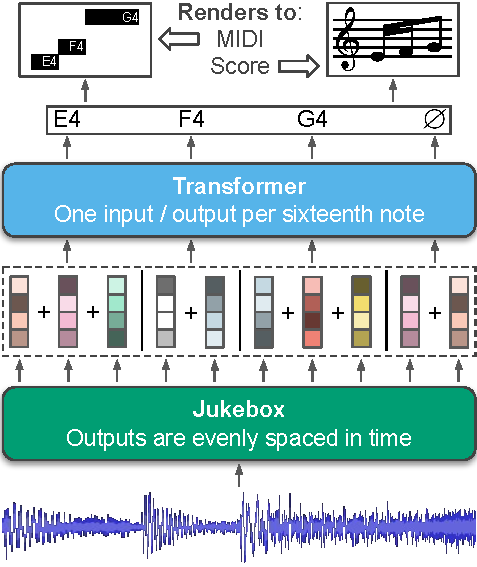
\includegraphics[width=8.1cm]{figs/fig1.pdf}
    \caption{
Our audio-to-score melody transcription approach involves 
(1)~extracting representations from Jukebox~\cite{dhariwal2020jukebox}, a generative model of music audio, 
(2)~averaging these representations across time to their nearest sixteenth note using \madmom~\cite{bock2016madmom,bock2016joint} for beat detection,
and
(3)~training a Transformer~\cite{vaswani2017attention} to detect melody note onsets (or rests) per sixteenth note.
}
 \label{fig:fig1}
\end{figure}

\begin{figure}
    \centering
    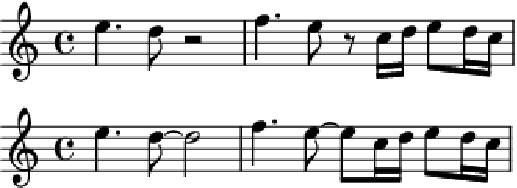
\includegraphics[width=8.1cm]{figs/heuristic_offsets.pdf}
    \caption{
The same note onsets engraved with ground truth~(top) vs. heuristic~(bottom) offsets. 
We argue that onset prediction suffices for producing human-readable melody transcriptions.
}
 \label{fig:heuristic_offsets}
\end{figure}

\begin{table}[]
    \centering
    \begin{tabular}{lcc}
\toprule
Features & $d$ & Onset F1 \\
\midrule
\mel{} & $229$ & $0.514$ \\
\mtthree{} & $512$ & $0.550$ \\
\jukebox{} & $4800$ & $0.615$ \\
\mel{}, \mtthree{} & $741$ & $0.548$ \\
\mel{}, \jukebox{} & $5029$ & $0.617$ \\
\mtthree{}, \jukebox{} & $5312$ & $0.622$ \\
\mel{}, \mtthree{}, \jukebox{} & $5541$ & $\mathbf{0.623}$ \\
\bottomrule
    \end{tabular}
    \caption{\hooktheory{} test set performance of different combinations of representations (when passed as input to train a Transformer). Different representations do contain complimentary information---combining all three yields highest performance---but Jukebox on its own is competitive with all combinations.}
    \label{tab:hooktheory_test}
\end{table}

\begin{table}[]
    \centering
    \begin{tabular}{lcc}
\toprule
 & Onset F1 & Onset F1 \\
Approach & \emph{Vox Only} & \emph{All} \\
\midrule
MT3 Zero-shot~\cite{gardner2021mt3} & $0.085$ & $0.133$ \\
Melodia~\cite{salamon2014melody} + Segmentation & $0.268$ & $0.201$ \\
DSP + HMM~\cite{ryynanen2008automatic} & $0.381$ & $0.420$ \\
Spleeter~\cite{hennequin2020spleeter} + Tony~\cite{mauch2015computer} & $0.462$ & $0.341$ \\
\midrule
\mel{} + Transformer & $0.621$ & $0.631$ \\
\mtthree{} + Transformer & $0.659$ & $0.701$ \\
\jukebox{} + Transformer & $\mathbf{0.786}$ & $\mathbf{0.744}$ \\
\bottomrule
    \end{tabular}
    \caption{Performance of different approaches on a small subset of \rwc~\cite{goto2002rwc,goto2003rwc,goto2004development}. The bottom three approaches were trained on the \hooktheory{} dataset as part of this work. We compute performance on both vocals and all melody instruments for fair comparison to baselines designed for vocal transcription.}
    \label{tab:rwc_ryy}
\end{table}


\bibliography{main}

\end{document}

